\documentclass[preprint,12pt]{elsarticle}
\usepackage{amssymb}
\usepackage{amsmath}
\usepackage[utf8]{inputenc}
\usepackage{color}
\usepackage{xcolor}
\usepackage[colorinlistoftodos,textsize=footnotesize]{todonotes}
\usepackage{tikz}
\usetikzlibrary{arrows.meta, patterns}
\usetikzlibrary{shapes, calc,quotes,angles}
\tikzset{%
  >={Latex[width=2mm,length=2mm]},
  % Specifications for style of nodes:
  base/.style = {
    rectangle, rounded corners, draw=black, minimum width=4cm, minimum
    height=1cm, text centered, font=\sffamily},
  decision/.style = {
    diamond, draw, rounded corners, fill=blue!20, minimum width=3cm, minimum height=0.5cm, text centered, font=\sffamily},
  activityStarts/.style = {base, fill=blue!30},
  startstop/.style = {base, fill=red!30},
  activityRuns/.style = {base, fill=green!30},
  process/.style = {
    base, minimum width=2.5cm, fill=orange!15, font=\ttfamily},
  state/.style={draw, circle, minimum size=0.8cm, inner sep=0pt},
  arrow/.style={-Stealth, shorten >=1pt},
  dot/.style={minimum size=4pt, inner sep=0pt, rounded corners=1pt, fill},
}

\newcommand{\ten}[1]{\ensuremath{\mathbf{#1}}}

\begin{document}

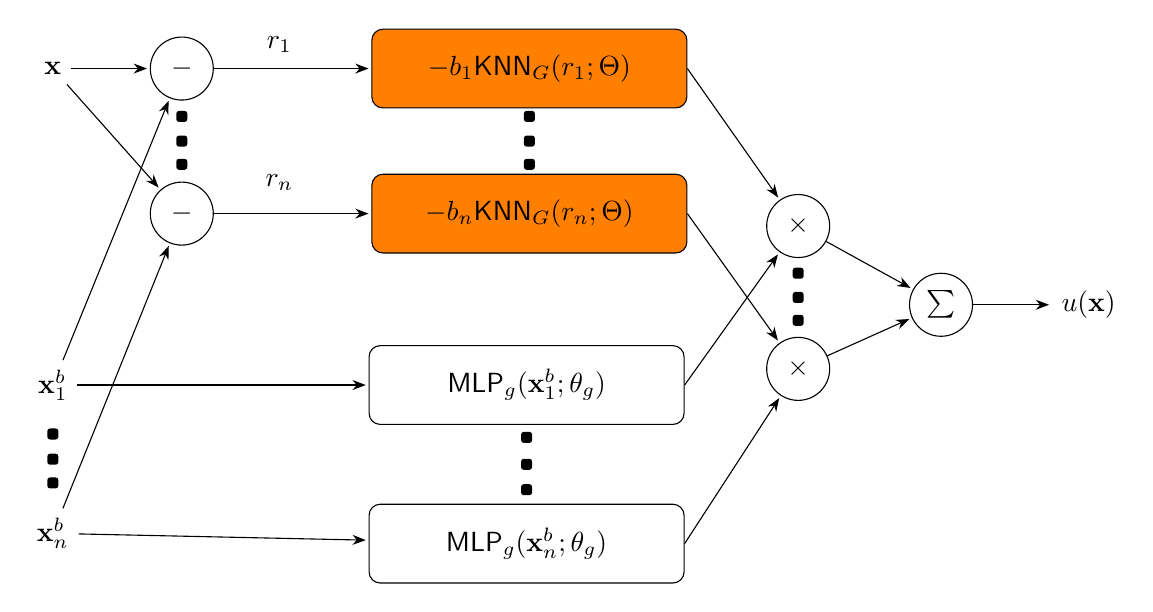
\begin{tikzpicture}
  \node[] (x1) {$\ten{x}$};
  \node[below =of x1, yshift=-2.5cm] (xc1) {$\ten{x}^b_1$};
  \node[below=of xc1, yshift=-0.25cm] (xc2) {$\ten{x}^b_n$};
  \node[dot] at ($(xc1)!0.33!(xc2)$) {};
  \node[dot] at ($(xc1)!0.5!(xc2)$) {};
  \node[dot] at ($(xc1)!0.66!(xc2)$) {};
  \node[state, right=of x1] (minus1) {$-$};
  \node[state, below=of minus1, yshift=-0.8] (minus2) {$-$};
  \node[right=of minus1, xshift=-0.45cm, yshift=0.3cm] (r1) {$r_1$};
  \node[below =of r1, yshift=-0.3cm] (r2) {$r_n$};
  \node[dot] at ($(minus1)!0.33!(minus2)$) {};
  \node[dot] at ($(minus1)!0.5!(minus2)$) {};
  \node[dot] at ($(minus1)!0.66!(minus2)$) {};
  \node[base, right=of minus1, xshift=1cm, fill=orange] (g1) {$-b_1\text{KNN}_G(r_1; \Theta)$};
  \node[base, right=of minus2, xshift=1cm, fill=orange] (g2) {$-b_n\text{KNN}_G(r_n; \Theta)$};
  \node[dot] at ($(g1)!0.33!(g2)$) {};
  \node[dot] at ($(g1)!0.5!(g2)$) {};
  \node[dot] at ($(g1)!0.66!(g2)$) {};
  \node[base, right=of xc1, xshift=2.7cm] (h1) {$\text{MLP}_g(\ten{x}_1^b; \theta_g)$};
  \node[base, below=of h1] (h2) {$\text{MLP}_g(\ten{x}_n^b; \theta_g)$};
  \node[dot] at ($(h1)!0.33!(h2)$) {};
  \node[dot] at ($(h1)!0.5!(h2)$) {};
  \node[dot] at ($(h1)!0.66!(h2)$) {};
  \node[state, right=of g1, yshift=-2.cm] (prod1) {$\times$};
  \node[state, below=of prod1] (prod2) {$\times$};
  \node[dot] at ($(prod1)!0.33!(prod2)$) {};
  \node[dot] at ($(prod1)!0.5!(prod2)$) {};
  \node[dot] at ($(prod1)!0.66!(prod2)$) {};
  \node[state, right=of prod1, yshift=-1cm] (int1) {$\sum$};
  \node[right=of int1] (out) {$u(\ten{x})$};
  \draw[arrow] (x1) -- (minus1);
  \draw[arrow] (xc1) -- (minus1);
  \draw[arrow] (x1) -- (minus2);
  \draw[arrow] (xc2) -- (minus2);
  \draw[arrow] (minus1) -- (g1);
  \draw[arrow] (minus2) -- (g2);
  \draw[arrow] (xc1) -- (h1.west);
  \draw[arrow] (xc2) -- (h2);
  \draw[arrow] (g1.east) -- (prod1);
  \draw[arrow] (h1.east) -- (prod1);
  \draw[arrow] (g2.east) -- (prod2);
  \draw[arrow] (h2.east) -- (prod2);
  \draw[arrow] (prod1) -- (int1);
  \draw[arrow] (prod2) -- (int1);
  \draw[arrow] (int1) -- (out);
\end{tikzpicture}

\end{document}